%-------------------------------------------------------------------------------
\documentclass{amsart}
\setlength{\textheight}{9in}
\setlength{\topmargin}{-0.25in}
\setlength{\textwidth}{7in}
\setlength{\evensidemargin}{-0.25in}
\setlength{\oddsidemargin}{-0.25in}
\usepackage{amsfonts}
\usepackage[utf8]{inputenc}
\usepackage[T1]{fontenc}
\usepackage{graphicx} 
\usepackage[export]{adjustbox}
\usepackage[section]{placeins}
% needed to include these graphics
%\graphicspath{{./Pictures/}}      % only in case you want to keep the pictures in a separate
                                  % subdirectory; also see the appropriate line below
\usepackage{caption}
\usepackage{subcaption}
\usepackage{float}
\usepackage{framed}
\newcounter{temp}
\theoremstyle{definition}
\newtheorem{Thm}{Theorem}
\newtheorem{Prob}{Problem}
\newtheorem*{Def}{Definition}
\newtheorem*{Ans}{Answer}
\newcommand{\dis}{\displaystyle}
\newcommand{\dlim}{\dis\lim}
\newcommand{\dsum}{\dis\sum}
\newcommand{\dint}{\dis\int}
\newcommand{\ddint}{\dint\!\!\dint}
\newcommand{\dddint}{\dint\!\!\dint\!\!\dint}
\newcommand{\dt}{\text{d}t}
\newcommand{\dA}{\text{d}A}
\newcommand{\dV}{\text{d}V}
\newcommand{\dx}{\text{d}x}
\newcommand{\dy}{\text{d}y}
\newcommand{\dz}{\text{d}z}
\newcommand{\dw}{\text{d}w}
\newcommand{\du}{\text{d}u}
\newcommand{\dv}{\text{d}v}
\newcommand{\ds}{\text{d}s}
\newcommand{\dr}{\text{d}r}
\newcommand{\dth}{\text{d}\theta}
\newcommand{\bbR}{\mathbb{R}}
\newcommand{\bbN}{\mathbb{N}}
\newcommand{\bbQ}{\mathbb{Q}}
\newcommand{\bbZ}{\mathbb{Z}}
\newcommand{\bbC}{\mathbb{C}}
\newcommand{\dd}[2]{\dfrac{\text{d}#1}{\text{d}#2}}
\newcommand{\dydx}{\dfrac{\text{d}y}{\text{d}x}}
\renewcommand{\labelenumi}{{\normalfont \arabic{enumi}.}}
\renewcommand{\labelenumii}{{\normalfont \alph{enumii}.}}
\renewcommand{\labelenumiii}{{\normalfont \roman{enumiii}.}}
\font \bggbf cmbx18 scaled \magstep2
\font \bgbf cmbx10 scaled \magstep2
\usepackage{fancyhdr}
\usepackage{lipsum}
\usepackage{amsmath}
\usepackage{empheq}
\newcommand*\widefbox[1]{\fbox{\hspace{2em}#1\hspace{2em}}}
% Clear the header and footer
\fancyhead{}
\fancyfoot{}
% Set the right side of the footer to be the page number
\rfoot{\thepage}
\fancyhf{}
\pagestyle{fancy}
%-------------------------------------------------------------------------------

\begin{document}

%-------------------------------------------------------------------------------
% HEADER INFO
\LARGE{CORPS-Group}
 
\large
John Boyington
\newline
\bigskip

%-------------------------------------------------------------------------------

\section{Device Description}
\bigskip

The device used in the experiment is a simple assembly consisting of gold foils embedded in HDPE sections contained within an aluminum tube.
Each 1 in. section of HDPE has a small hole drilled into one side where a 5 mm OD disk of gold foil is inserted.
Eleven of these sections are assembled and contained within the aluminum tubing (0.75" OD).
The device is inserted such that the first foil illuminated by the beam is not covered.
Below are images of the response functions associated with the device.

\begin{figure}[!htb]
\centering
\begin{subfigure}{.5\textwidth}
  \centering
  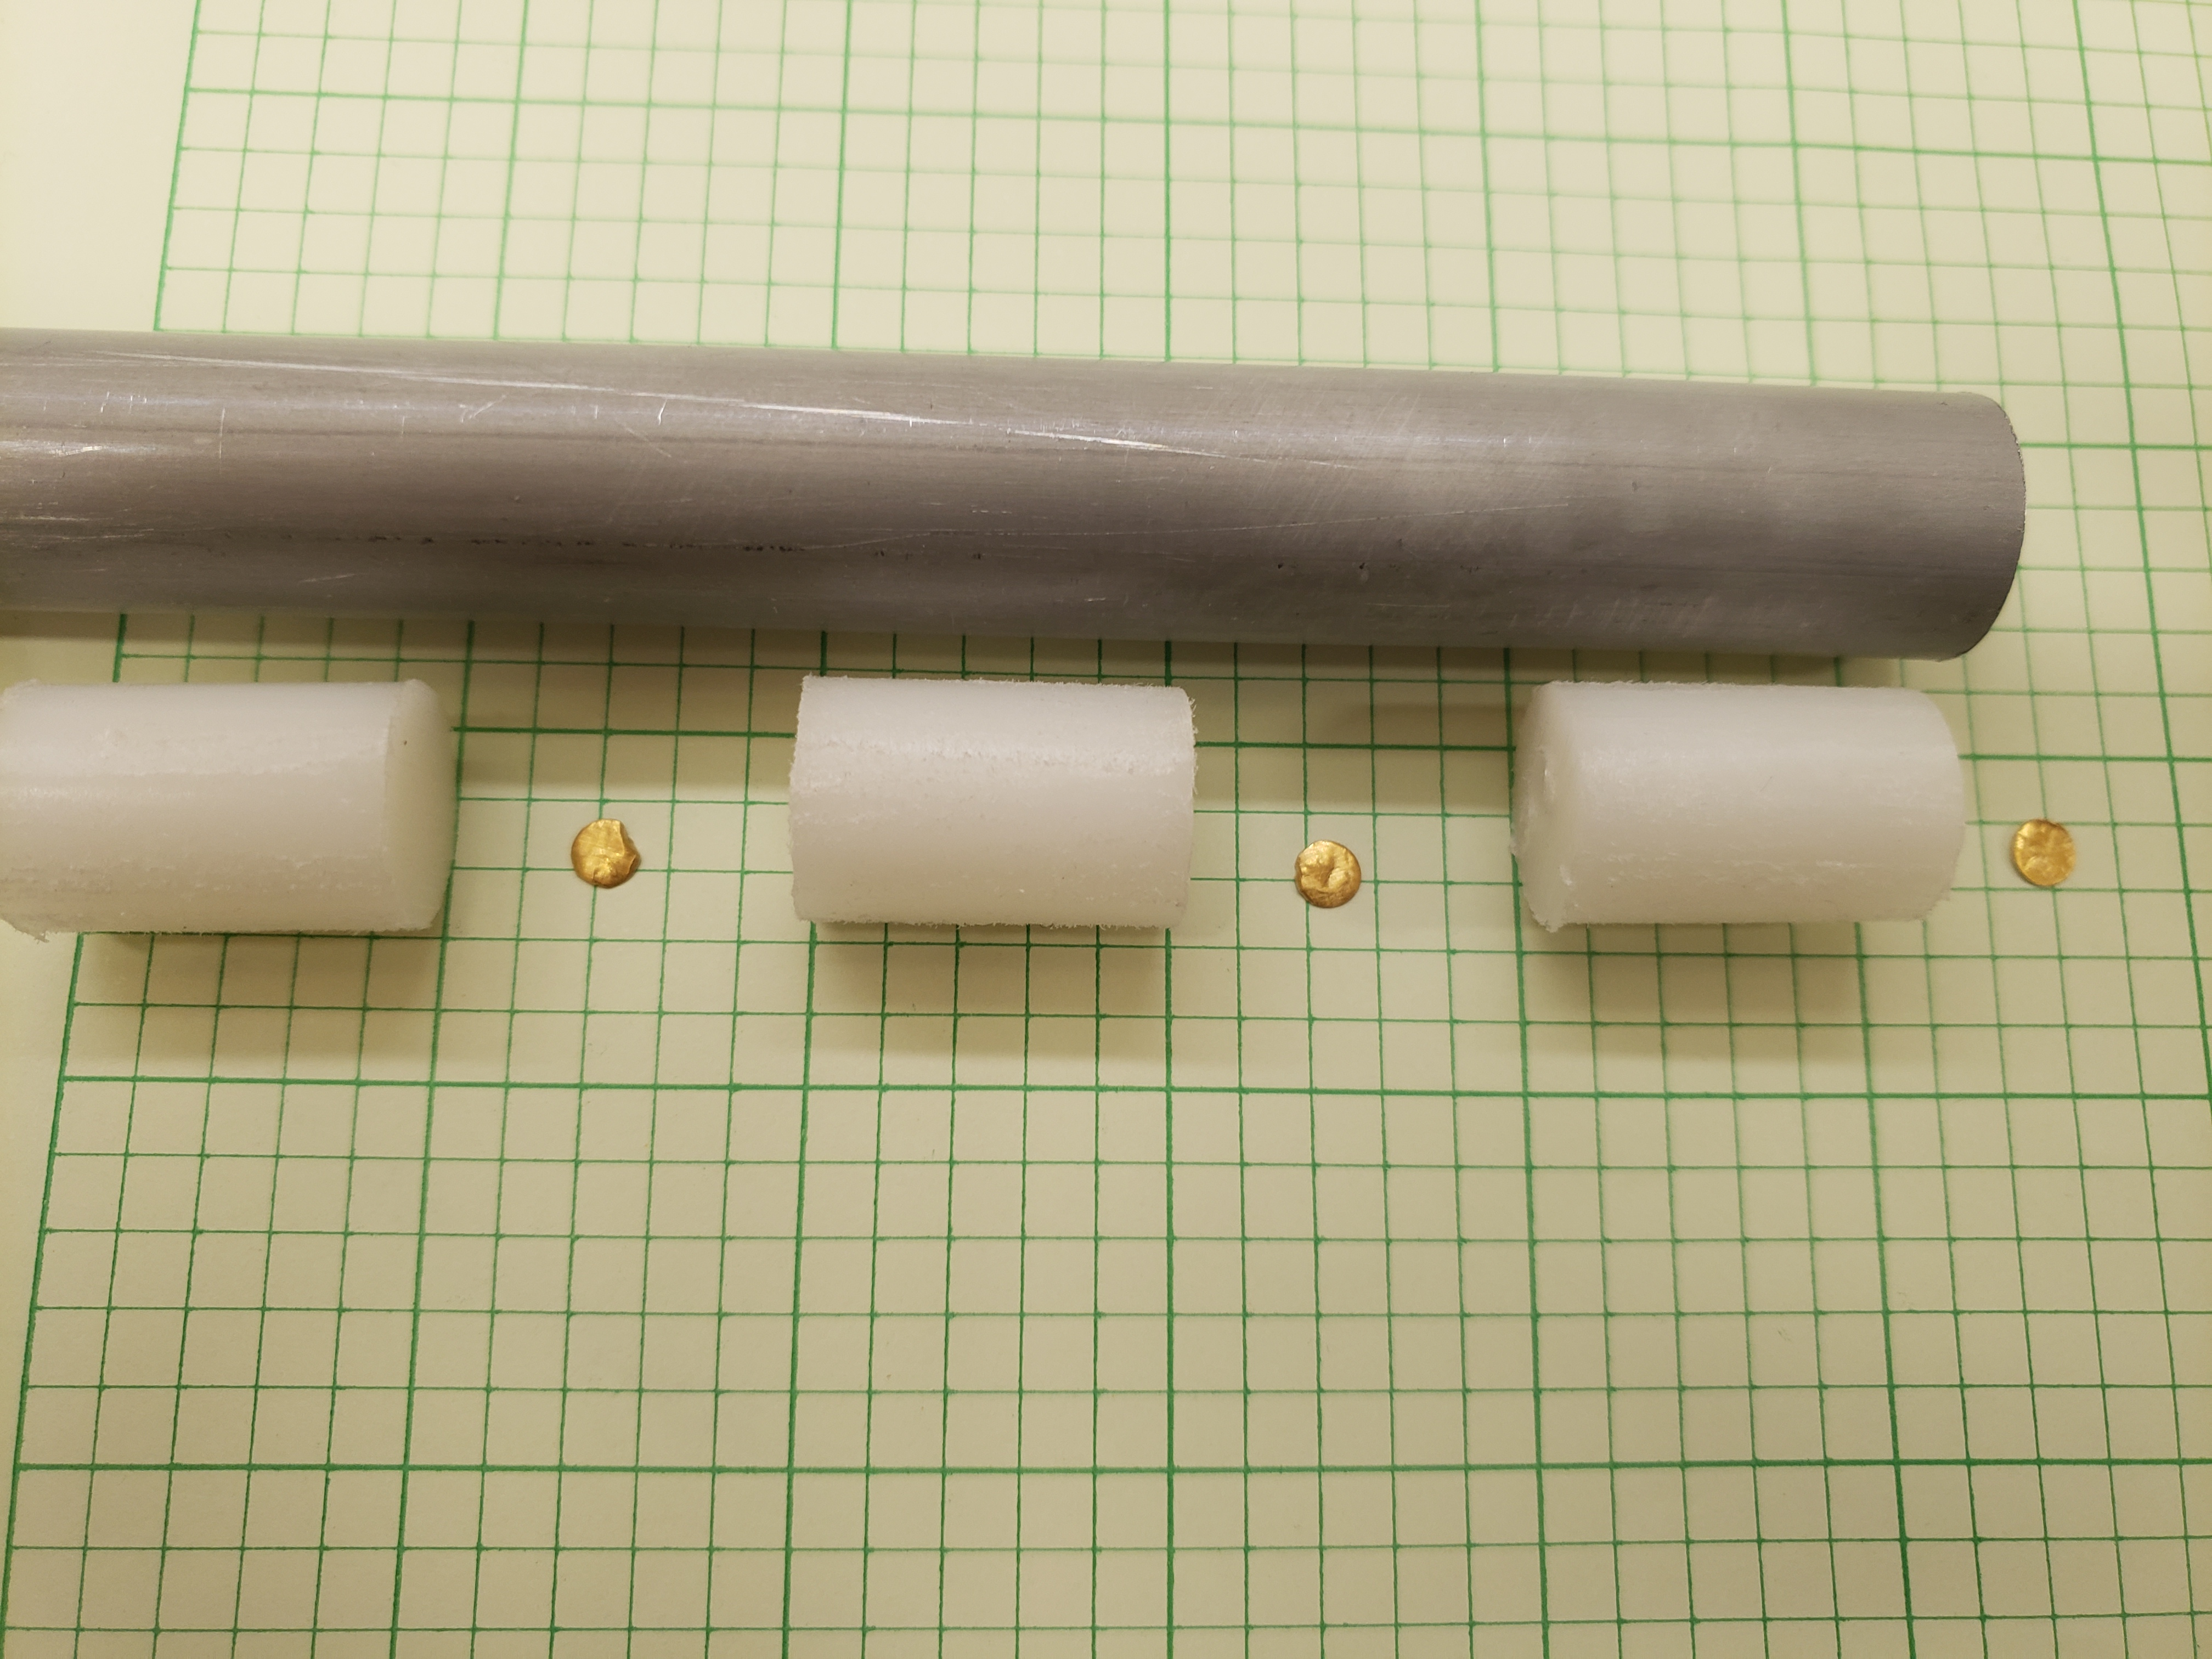
\includegraphics[width=.8\linewidth]{img/exploded.jpg}
  \caption{An exploded look at the device.}
\end{subfigure}%
\begin{subfigure}{.5\textwidth}
  \centering
  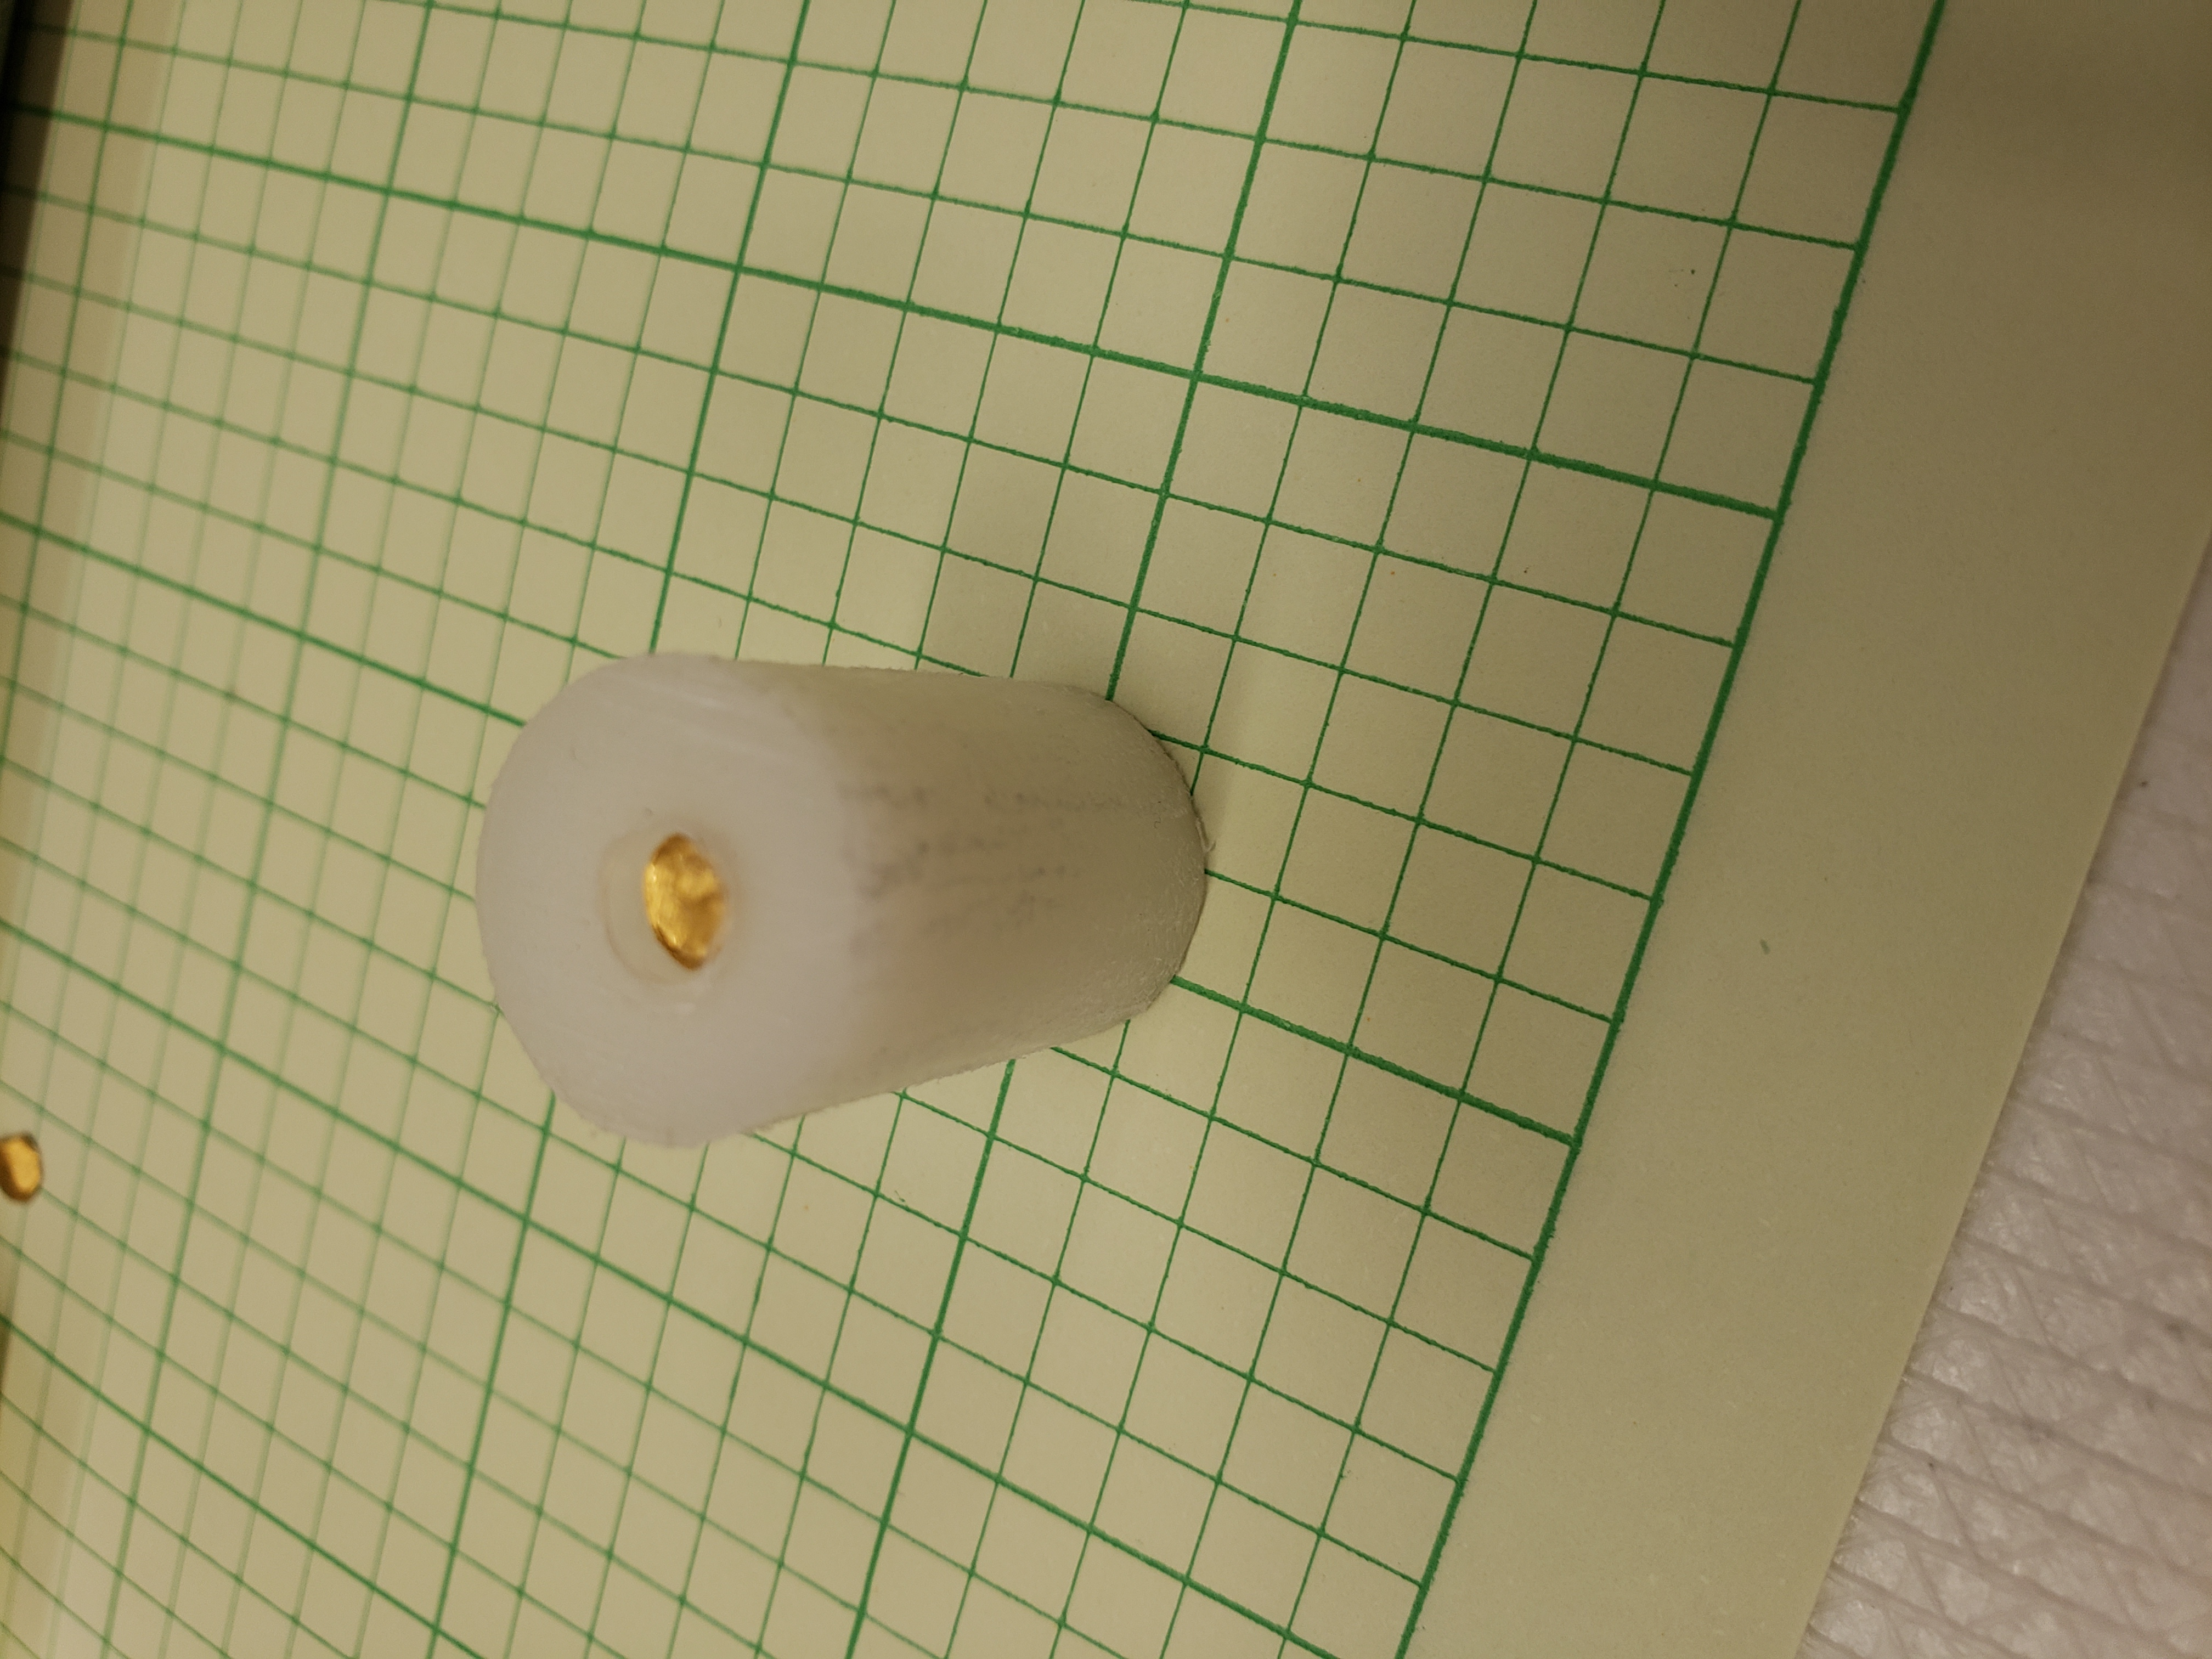
\includegraphics[width=.8\linewidth]{img/section0.jpg}
  \caption{One section of HDPE with foil inserted.}
\end{subfigure}
\end{figure}


\begin{figure}[!htb]
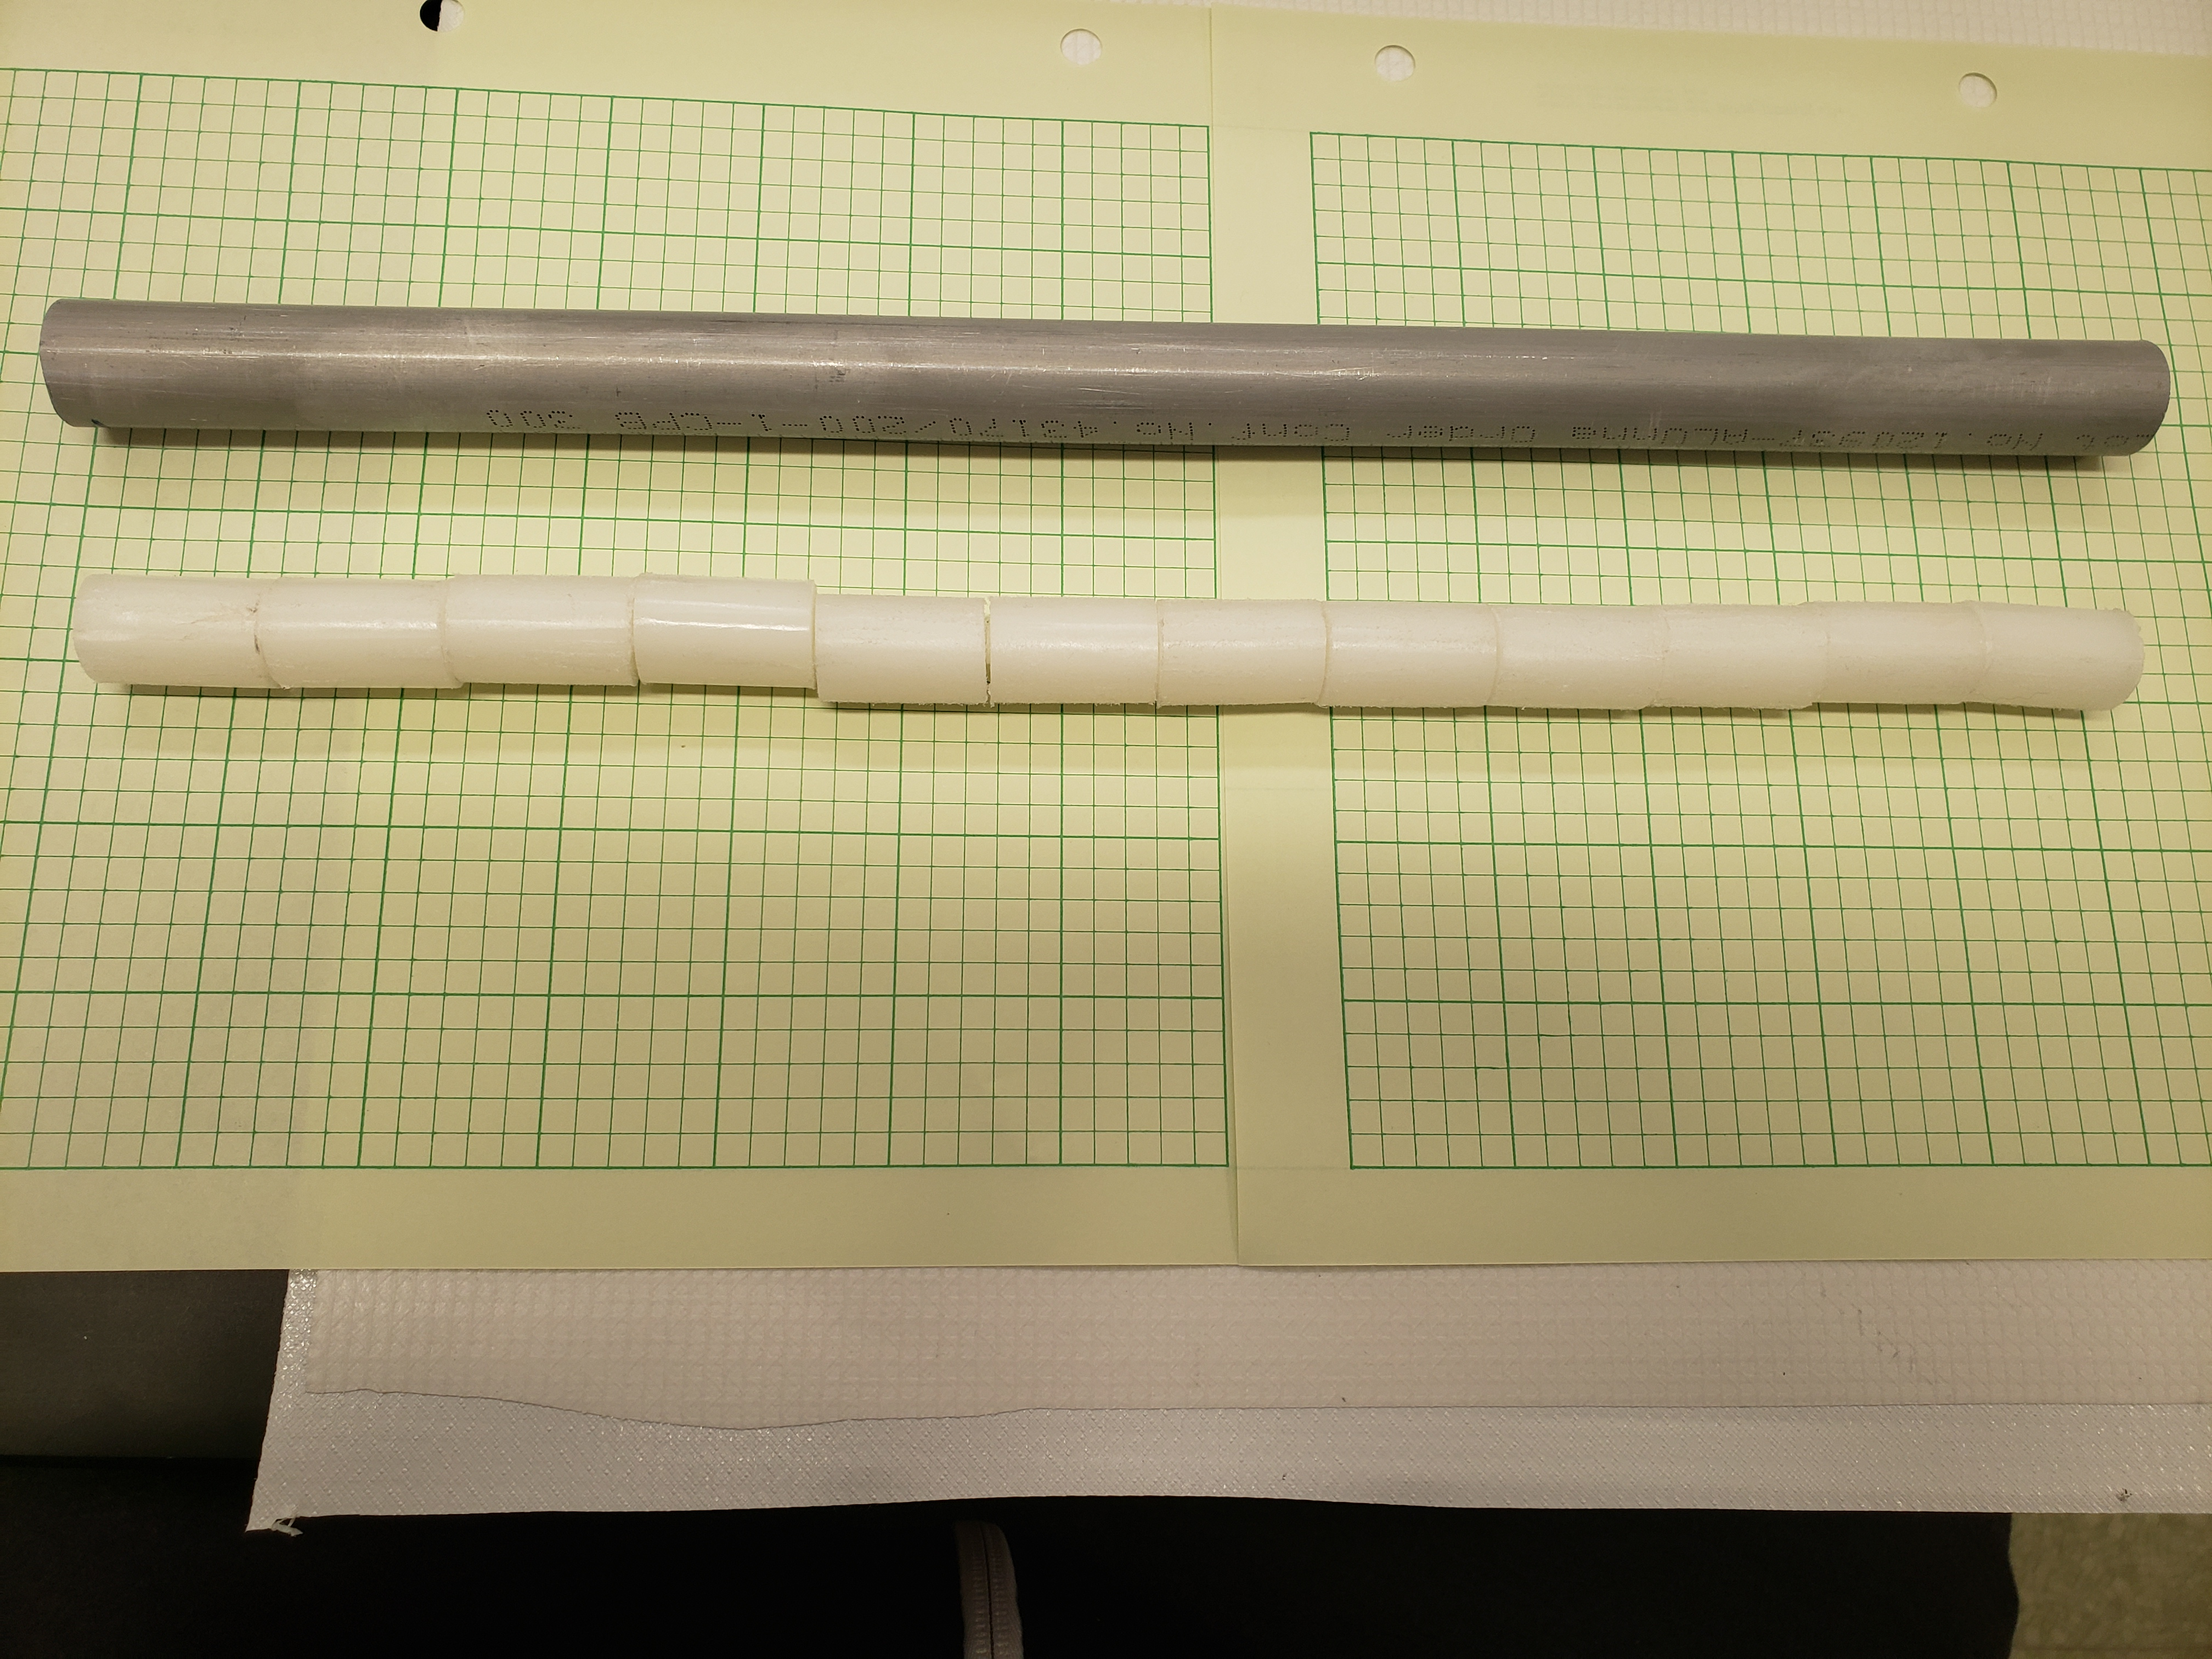
\includegraphics[width=0.6\linewidth]{img/assy0.jpg}
\caption{A look at semi-assembled internals. Note: the full device will have only 11 sections, not the 12 depicted.}
\end{figure}

\begin{figure}[!htb]
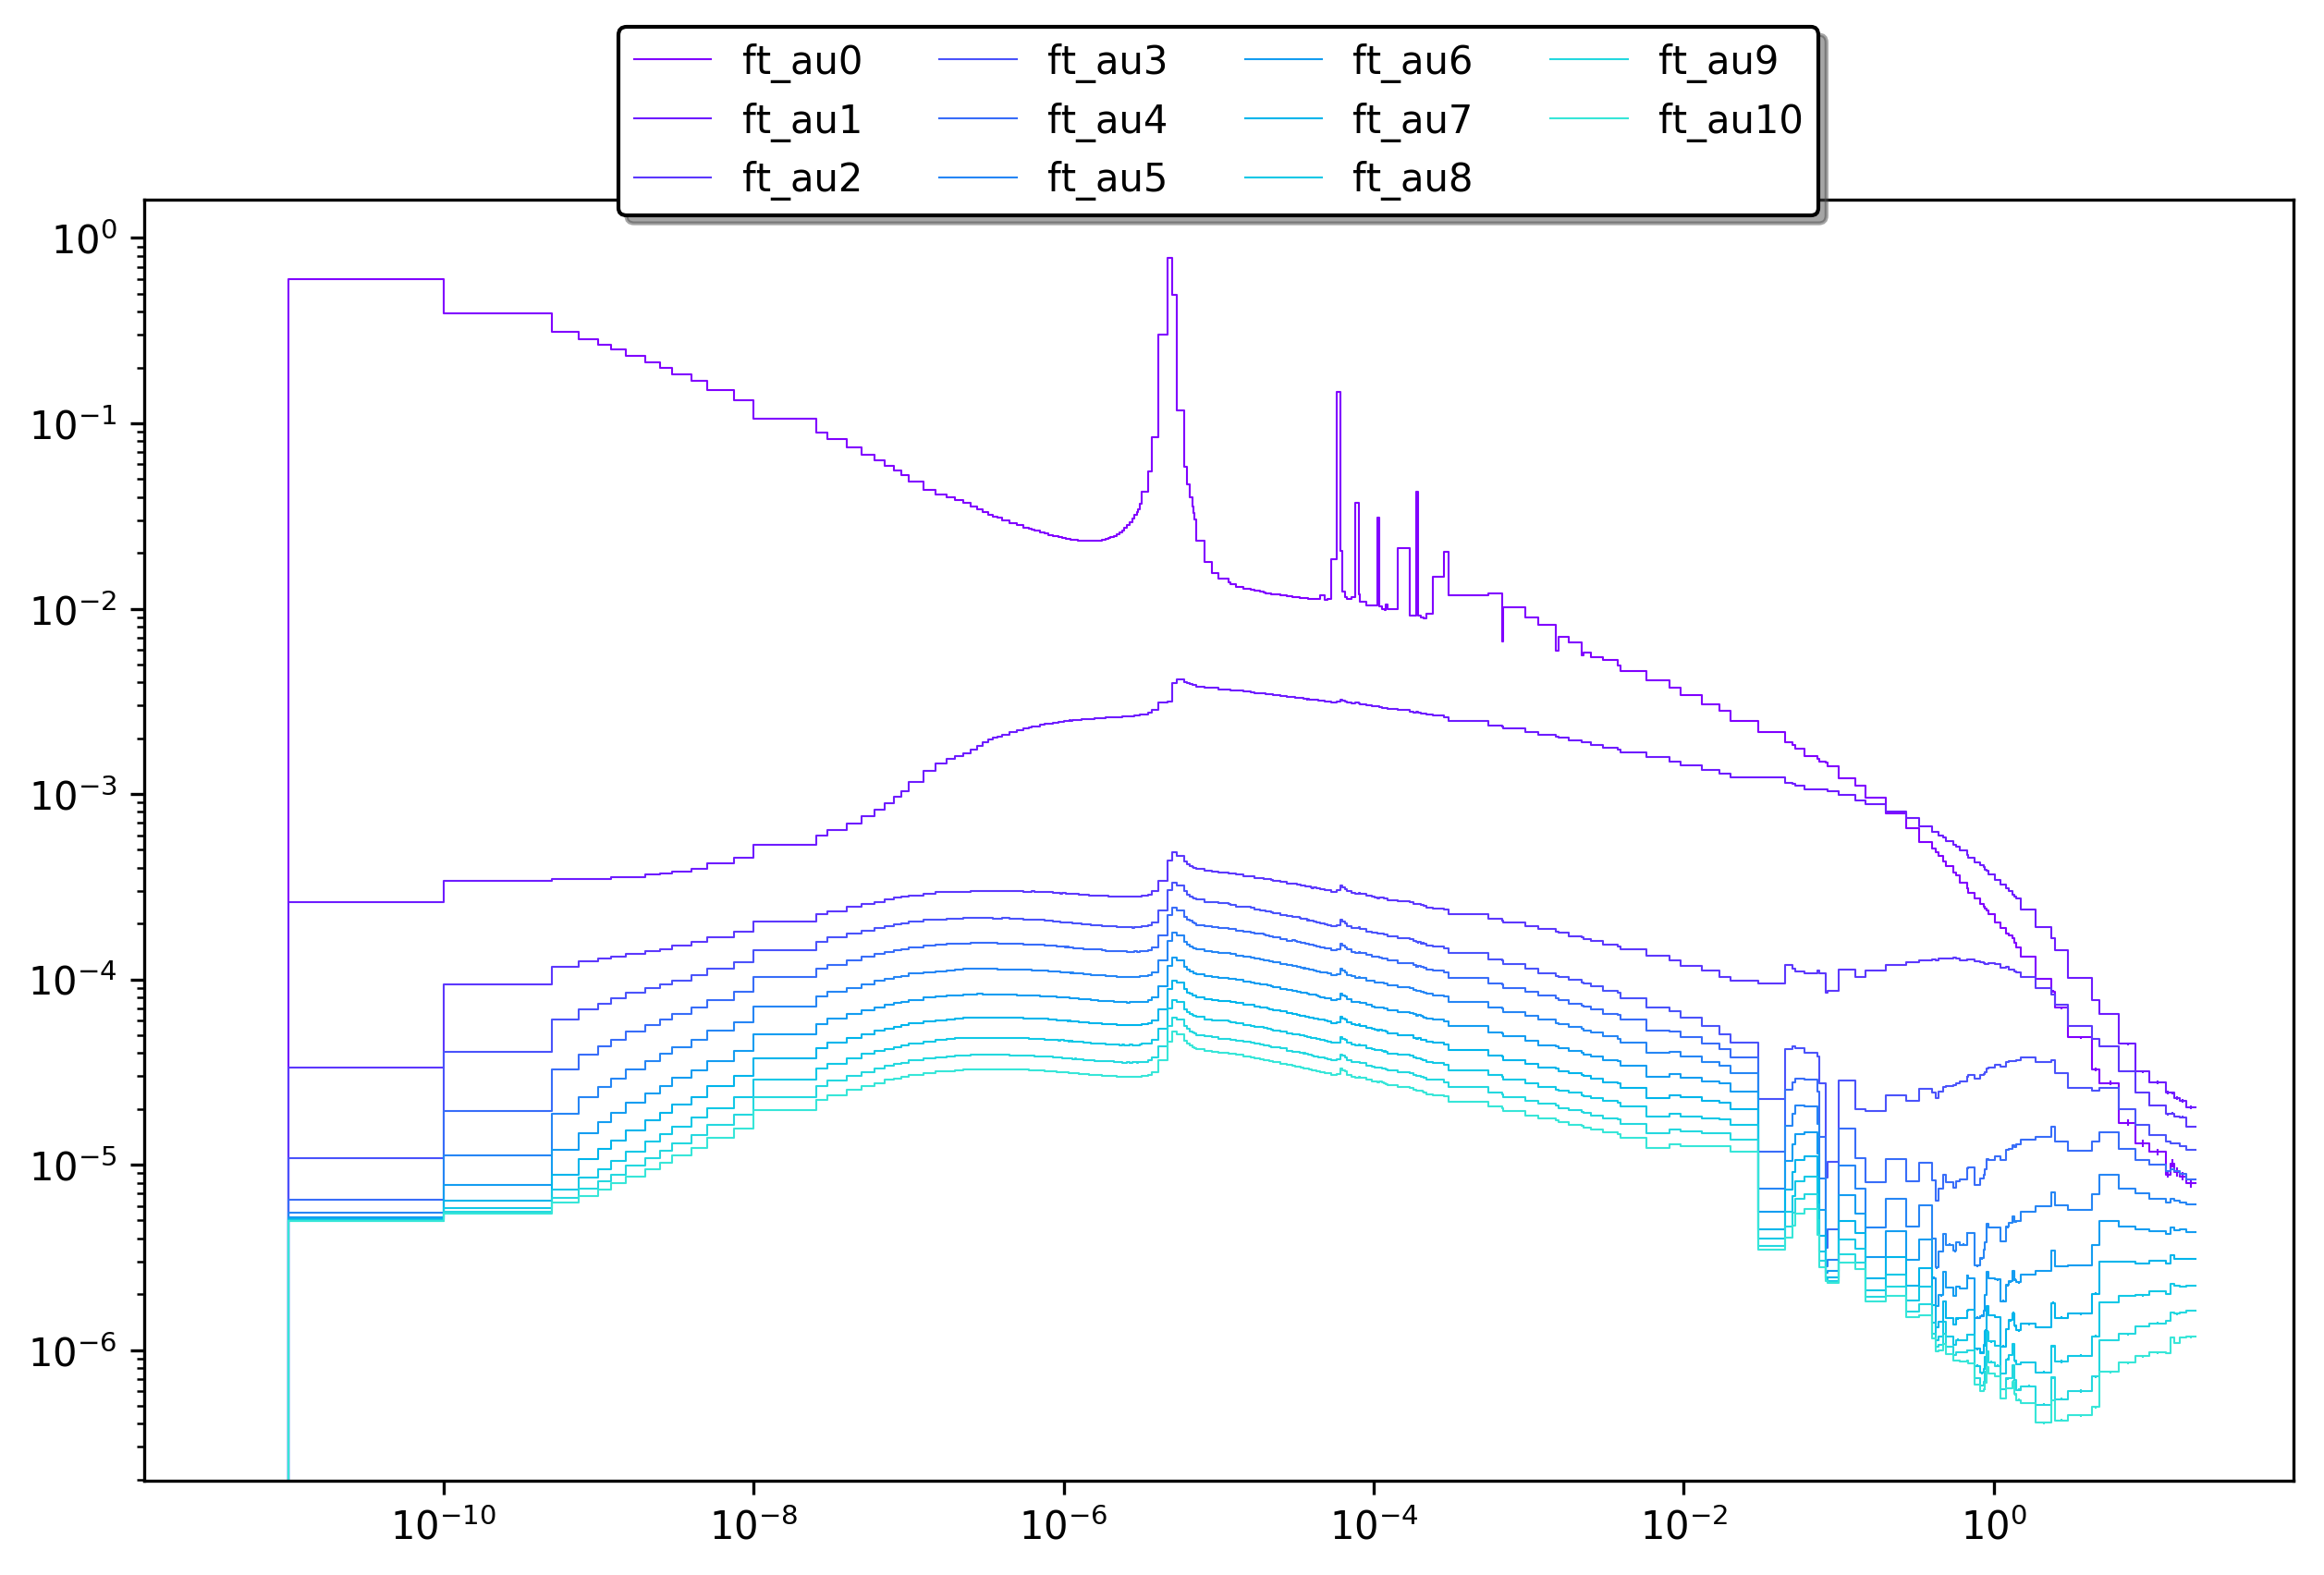
\includegraphics[width=0.8\linewidth]{../response/plot/ft_au.png}
\caption{Response functions associated with each foil.}
\end{figure}

\begin{figure}[!htb]
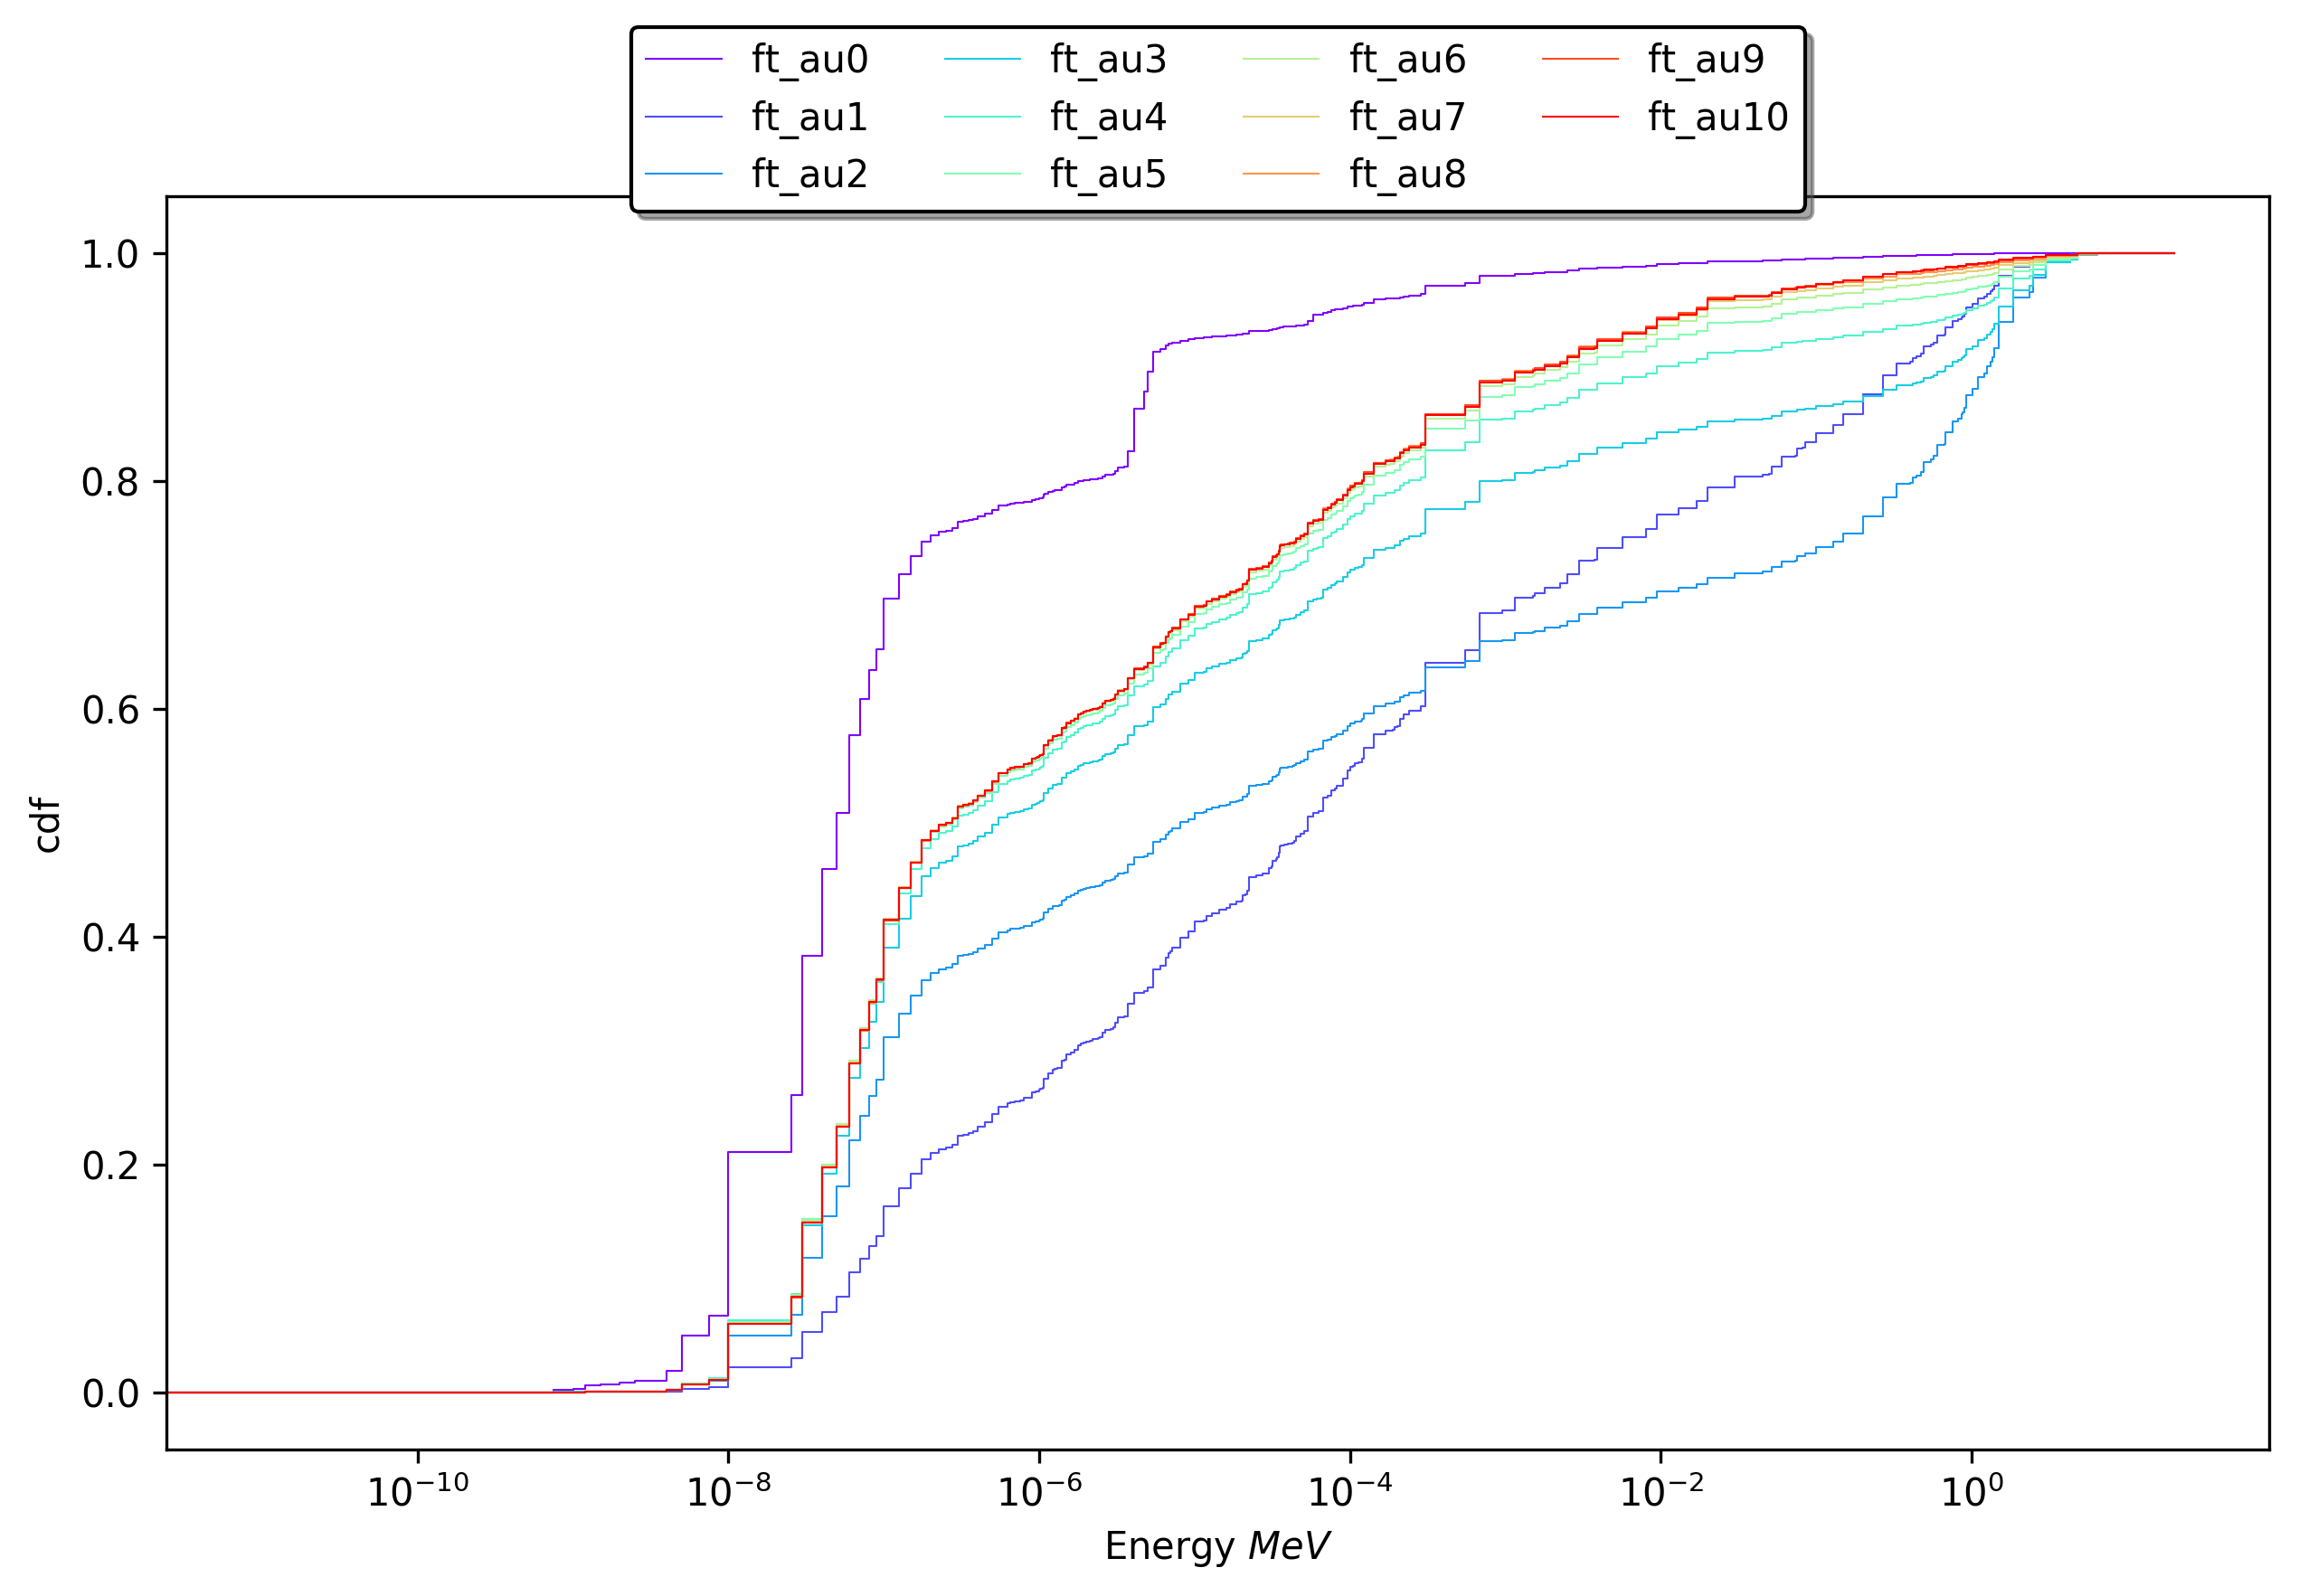
\includegraphics[width=0.8\linewidth]{../response/plot/ft_au_cdf.png}
\caption{Cumulative distribution function of each foil multiplied by the expected integral flux.}
\end{figure}


\clearpage

\section{Experimental Procedures}
\bigskip

\noindent
This section contains a description of the experiment to be run on 4/5/19. \\
Power Level: 100 kW(th) \\
Irradiation Time: 3 hours \\
FT: Foil Tube \\
NEBP: Northeast Beam Port \\


\begin{enumerate}
\item Assemble FT.
\item Disassemble NEBP shielding.
\item Insert FT into the NEBP far enough to ensure alignment. Majority of tube should be situated outside of NEBP (ideally, ~1 in. inserted).
\item Measure extruded portion of FT and record value.
\item Evacuate location around NEBP.
\item Reactor is brought to nominal power.
\item Nominal power is maintained for nominal irradiation time.
\item Following irradiation, shutdown reactor.
\item Measurement is taken of FT radioactivity and recorded.
\item FT is removed from NEBP. Record absolute time.
\item Rod is used to push each FT HDPE section and foil into respective, numbered bag.
\item Bags are collected and taken to NAA lab.
\item Foils are removed from HDPE section counted from lowest to highest activity using HPGe detector.
\item After counting, foils are moved to storage location where they are kept to decay.
\item All files are transferred to {\tt nebp/} repository.
\end{enumerate}


\newpage
\section{Expected Results}
\bigskip

The image below contains information on the expected responses of each foil.
The largest predicted activity, the bare foil is 54.19 $\mu Ci$.
The lowest predicted activity, the foil farthest from the beam is 0.0292 $\mu Ci$.

\begin{figure}[!htb]
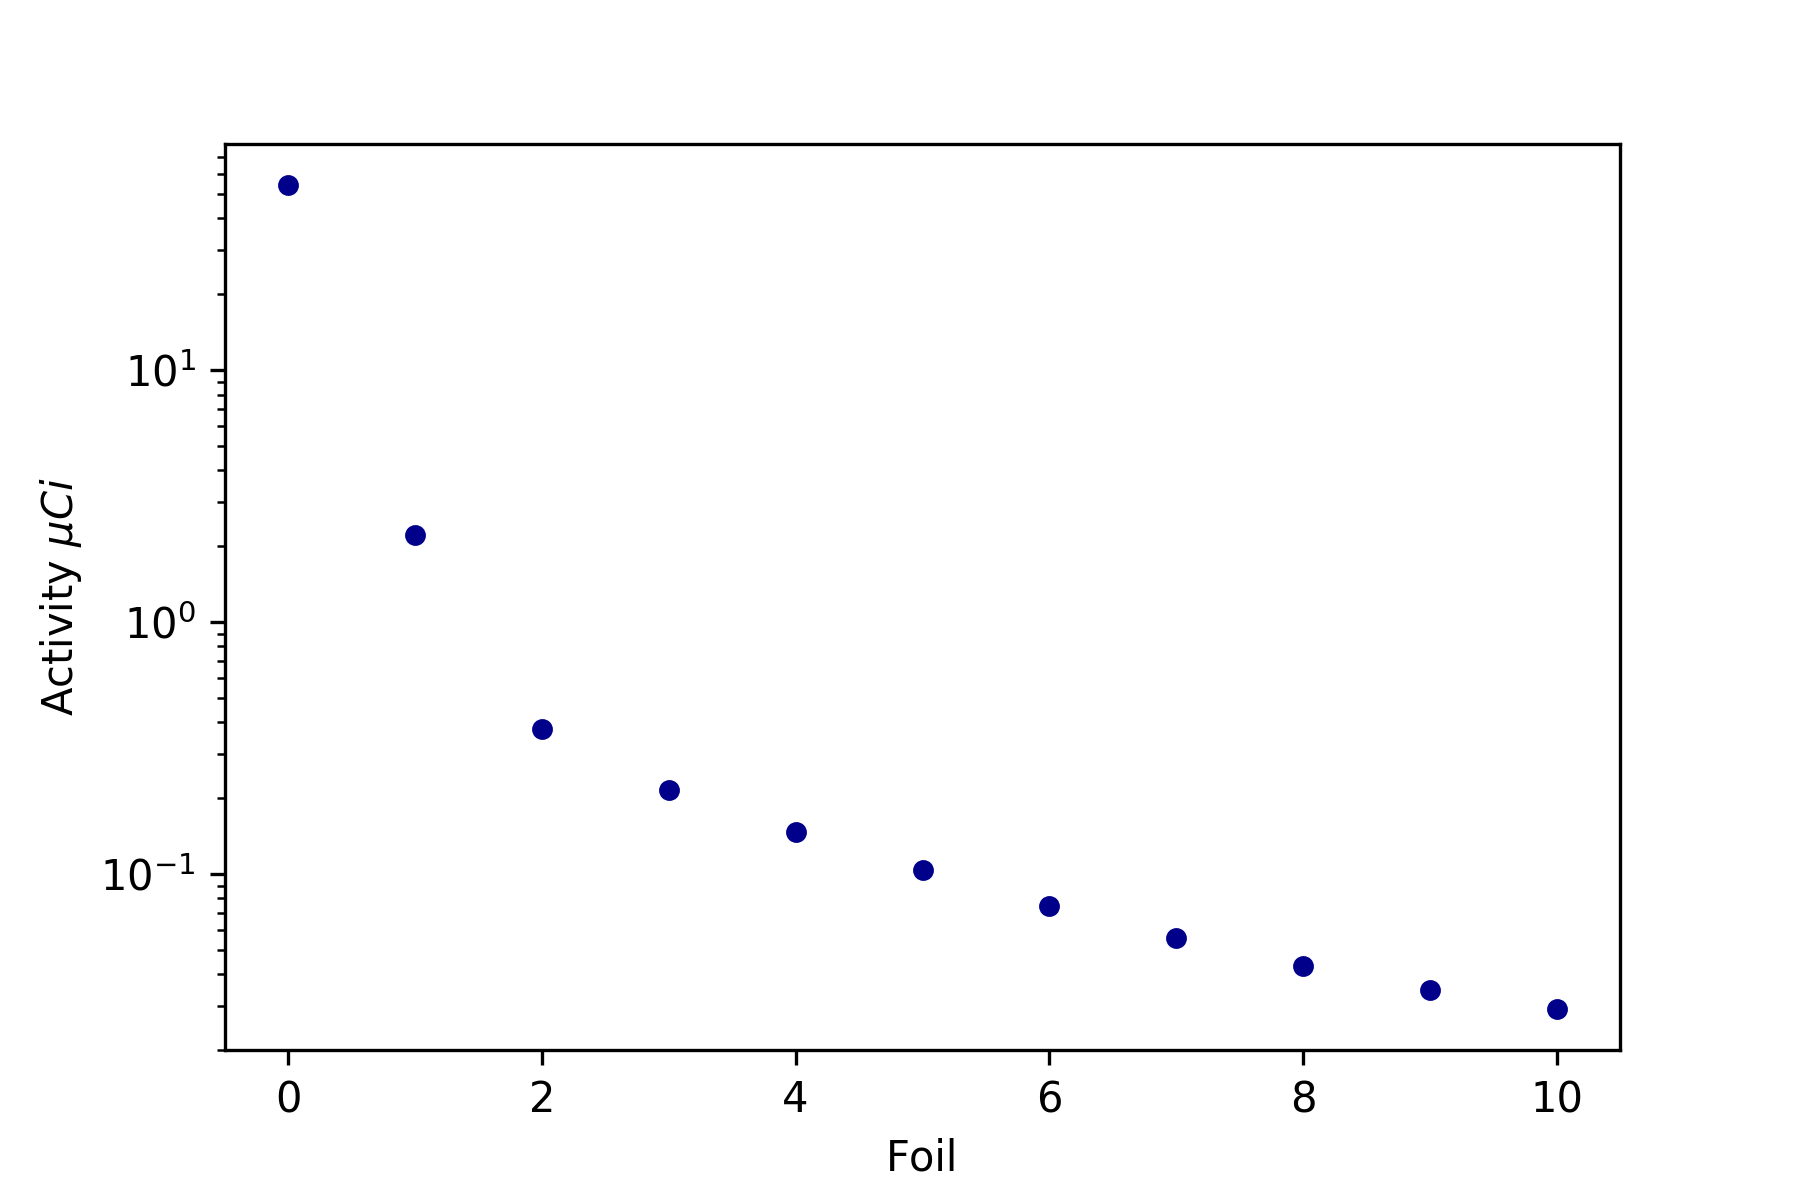
\includegraphics[width=0.8\linewidth]{../response/plot/ft_au_theoretical_responses.png}
\caption{The expected activites of each foil following the irradiation.}
\end{figure}

\end{document}

